\documentclass[11pt,prb,aps,nofootinbib,superscriptaddress,floatfix]{revtex4-2}
\usepackage{graphicx}
\usepackage{xcolor}
\usepackage{amsmath}
\usepackage{amssymb}
\usepackage{natmove}
\usepackage{natbib}
\usepackage{hyperref}
\usepackage{bm}

\begin{document}

\title{The Mechanism of Shrimpoluminescence}

\author{Tyler C. Sterling}
\email{ty.sterling@colorado.edu}
%\affiliation{Department of Physics, University of Colorado at Boulder, Boulder, Colorado 80309, USA}

\date{\today}

\begin{abstract}
Snapping shrimp produce bubbles that emit light when they collapse. When a bubble collapses so strongly that it emits light, the light emission is usually called sonoluminescence. In the case of the shrimp, the light emission is called \emph{shrimpoluminescence}. The bubble collapses so fast that no heat can escape and the gas trapped in the bubble becomes hot enough to ionize. Light is emitted through electron-ion bremsstrahlung, electron-atom bremsstrahlung, and electron-ion recombination. In this paper, we study the dynamics of a sonoluminescing bubble and learn how to calculate the spectrum of emitted light, allowing us to explain the physical mechanisms of shrimpoluminescence.
\end{abstract}

\maketitle

\section{Introduction}

Snapping shrimp, like our cute friend in Fig. \ref{fig:shrimp}, produce cavitating bubbles by snapping their claws \cite{versluis2000snapping,lohse2001snapping,tang2019bioinspired}. They have a strong appendage called the \emph{dactyl} [Fig. \ref{fig:shrimp} (center)] that is used to create a high-velocity jet of water. The low pressure region in the jet's wake forms a bubble [Fig. \ref{fig:shrimp} (right)] that, when it collapses, produces a noise loud enough to be detected over a mile away \cite{everest1948acoustical}. The sound wave produced by the collapsing bubble is used to stun or kill prey \cite{versluis2000snapping}. If the shrimp's prey had very sensitive eyes (and also were not dead) they might notice a flash of light is also produced through an effect known as ``shrimpoluminescence" in the case of the shrimp \cite{lohse2001snapping}, but more generally called \emph{sonoluminescence}.
%The noise produced by groups of shrimp is so intense that the U.S. Navy used them as ``sonar-camouflage" in the Pacific ocean during World War II \cite{versluis2000snapping}. The shrimp were not patriots helping the war-effort however; they snapped for food. The sound wave produced by the cavitating bubble is used to stun or kill prey \cite{versluis2000snapping}. If the shrimp's prey had very sensitive eyes (and also were not dead) they might notice a flash of light is also produced through an effect referred to as ``shrimpoluminescence" in the case of the shrimp \cite{lohse2001snapping}, but more generally known as \emph{sonoluminescence}.

\begin{figure}
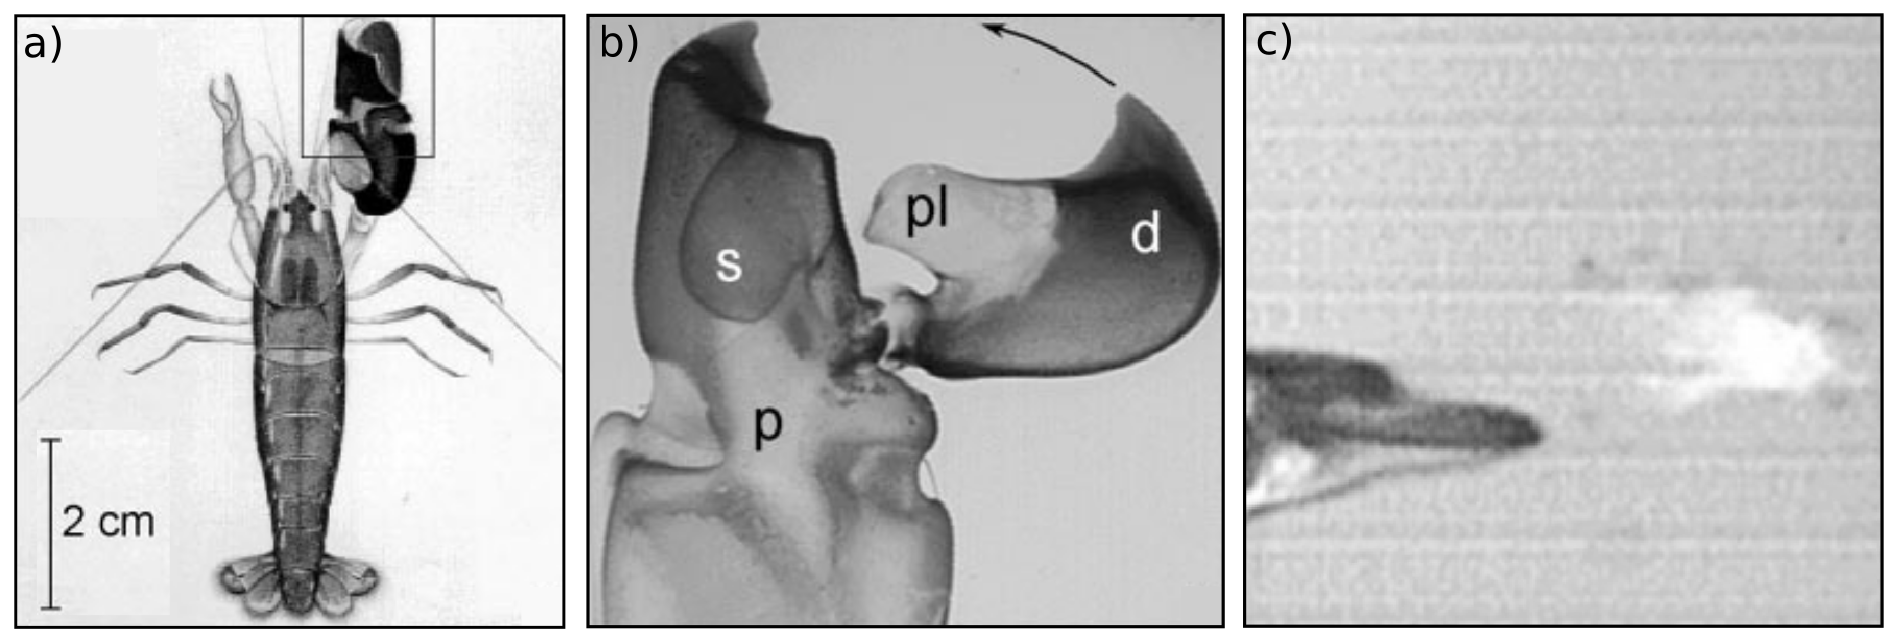
\includegraphics[width=0.85\linewidth]{figs/shrimp.pdf}
    \caption{(left) Snapping shrimp (\emph{Alpheus heterochaelis}). (center) Blown-up view of the shrimp's claw. The \emph{plunger} (pl) on the \emph{dactyl} (d) rapidly enters the \emph{socket} (s), ejecting a high-velocity jet of water. A time near the bubble collapse is shown on the right. The light emission is too dim to be seen by the naked eye. Adapted from refs. \cite{versluis2000snapping} and \cite{lohse2001snapping}.}
\label{fig:shrimp}
\end{figure}

Sonoluminescence (SL) is defined as the process by which a ``driven gas bubble collapses so strongly that the energy focusing at collapse leads to light emission" \cite{brenner2002single}. SL comes in two forms: (i) single-bubble sonoluminescence and (ii) multi-bubble sonoluminescence. Multi-bubble sonoluminescence (MBSL) consists of  ``the simultaneous creation and destruction of many separate, individual cavitation bubbles" \cite{crum1994sonoluminescence,brenner2002single}. In single-bubble sonoluminescence (SBSL), rather obviously, only a single bubble is present \cite{gaitan1992sonoluminescence}. In contrast to MBSL, there are no other bubbles present for the emitted light to scatter from. Similarly, the bubble does not interact with other bubbles and, due to its tiny extent, does not interact with the container walls. Both theory and experiments are greatly simplified compared to MBSL. Practically all progress on understanding SL has come from SBSL, with some authors even calling it ``the hydrogen atom of sonoluminescence" \cite{lohse2018bubble,crum1994sonoluminescence}. 

With this in mind, let's use SBSL as an idealization of shrimpoluminescence. The discussion will be much simpler if we further specialize to \emph{stable} SBSL. In stable SBSL the bubble is driven to produce light but does not disappear after collapsing; rather, it is periodically driven and emits light every cycle. This is in contrast to shrimpoluminescence, where the bubble is transient; i.e. it disappears after emitting light. The significance of this contradiction is addressed later.

In a SBSL\footnote{From here on,``SBSL" means \emph{stable} SBSL unless explicitly specified.} experiment, a bubble filled with noble-gas is trapped at the center of a flask containing water [Fig. \ref{fig:summary_fig} (a)]. A transducer is connected to the flask and is tuned to excite one of its vibrational modes. The flask's oscillations induce oscillating pressure in the fluid, $P(t)$, shown as a function of time in Fig. \ref{fig:summary_fig} (b). The oscillating pressure drives the bubble's expansion/contraction. For just the right driving pressure, we get the complicated behavior of the bubble's radius, $R(t)$, shown in Fig. \ref{fig:summary_fig} (b). To understand how these dynamics lead to SBSL, let's look at the blown-up snapshots of the bubble at the times $t_1$, $t_2$ and $t_3$:
\begin{itemize}
    \item [$\bm{t}$=$\bm{t_1}$] The driving pressure in the fluid is negative and the bubble is expanding. Surface-tension opposes the driving pressure, slowing the bubble's expansion.
    \item [$\bm{t}$=$\bm{t_2}$] The driving pressure is now positive and the bubble's radius is very large. The gas is dilute and offers little resistance to compression. Surface-tension works with the positive driving pressure to shrink the bubble: the bubble violently collapses in a process called \emph{cavitation}. 
    \item [$\bm{t}$=$\bm{t_3}$] The bubble is at its minimum radius. During cavitation, the gas was compressed so quickly that heat could not flow out of the bubble. For a very short time ($ 0.003\% $ of the bubble's cycle \cite{suslick2008inside}), the temperature in the bubble can reach $10,000-30,000$ K \cite{an2006mechanism,hilgenfeldt1999simple,an2008spectral,an2009diagnosing}. This is when light is emitted from the bubble. After the light pulse, there is a period of ``after-bouncing" until the driving pressure becomes negative and the cycle begins again.
\end{itemize}


\begin{figure}
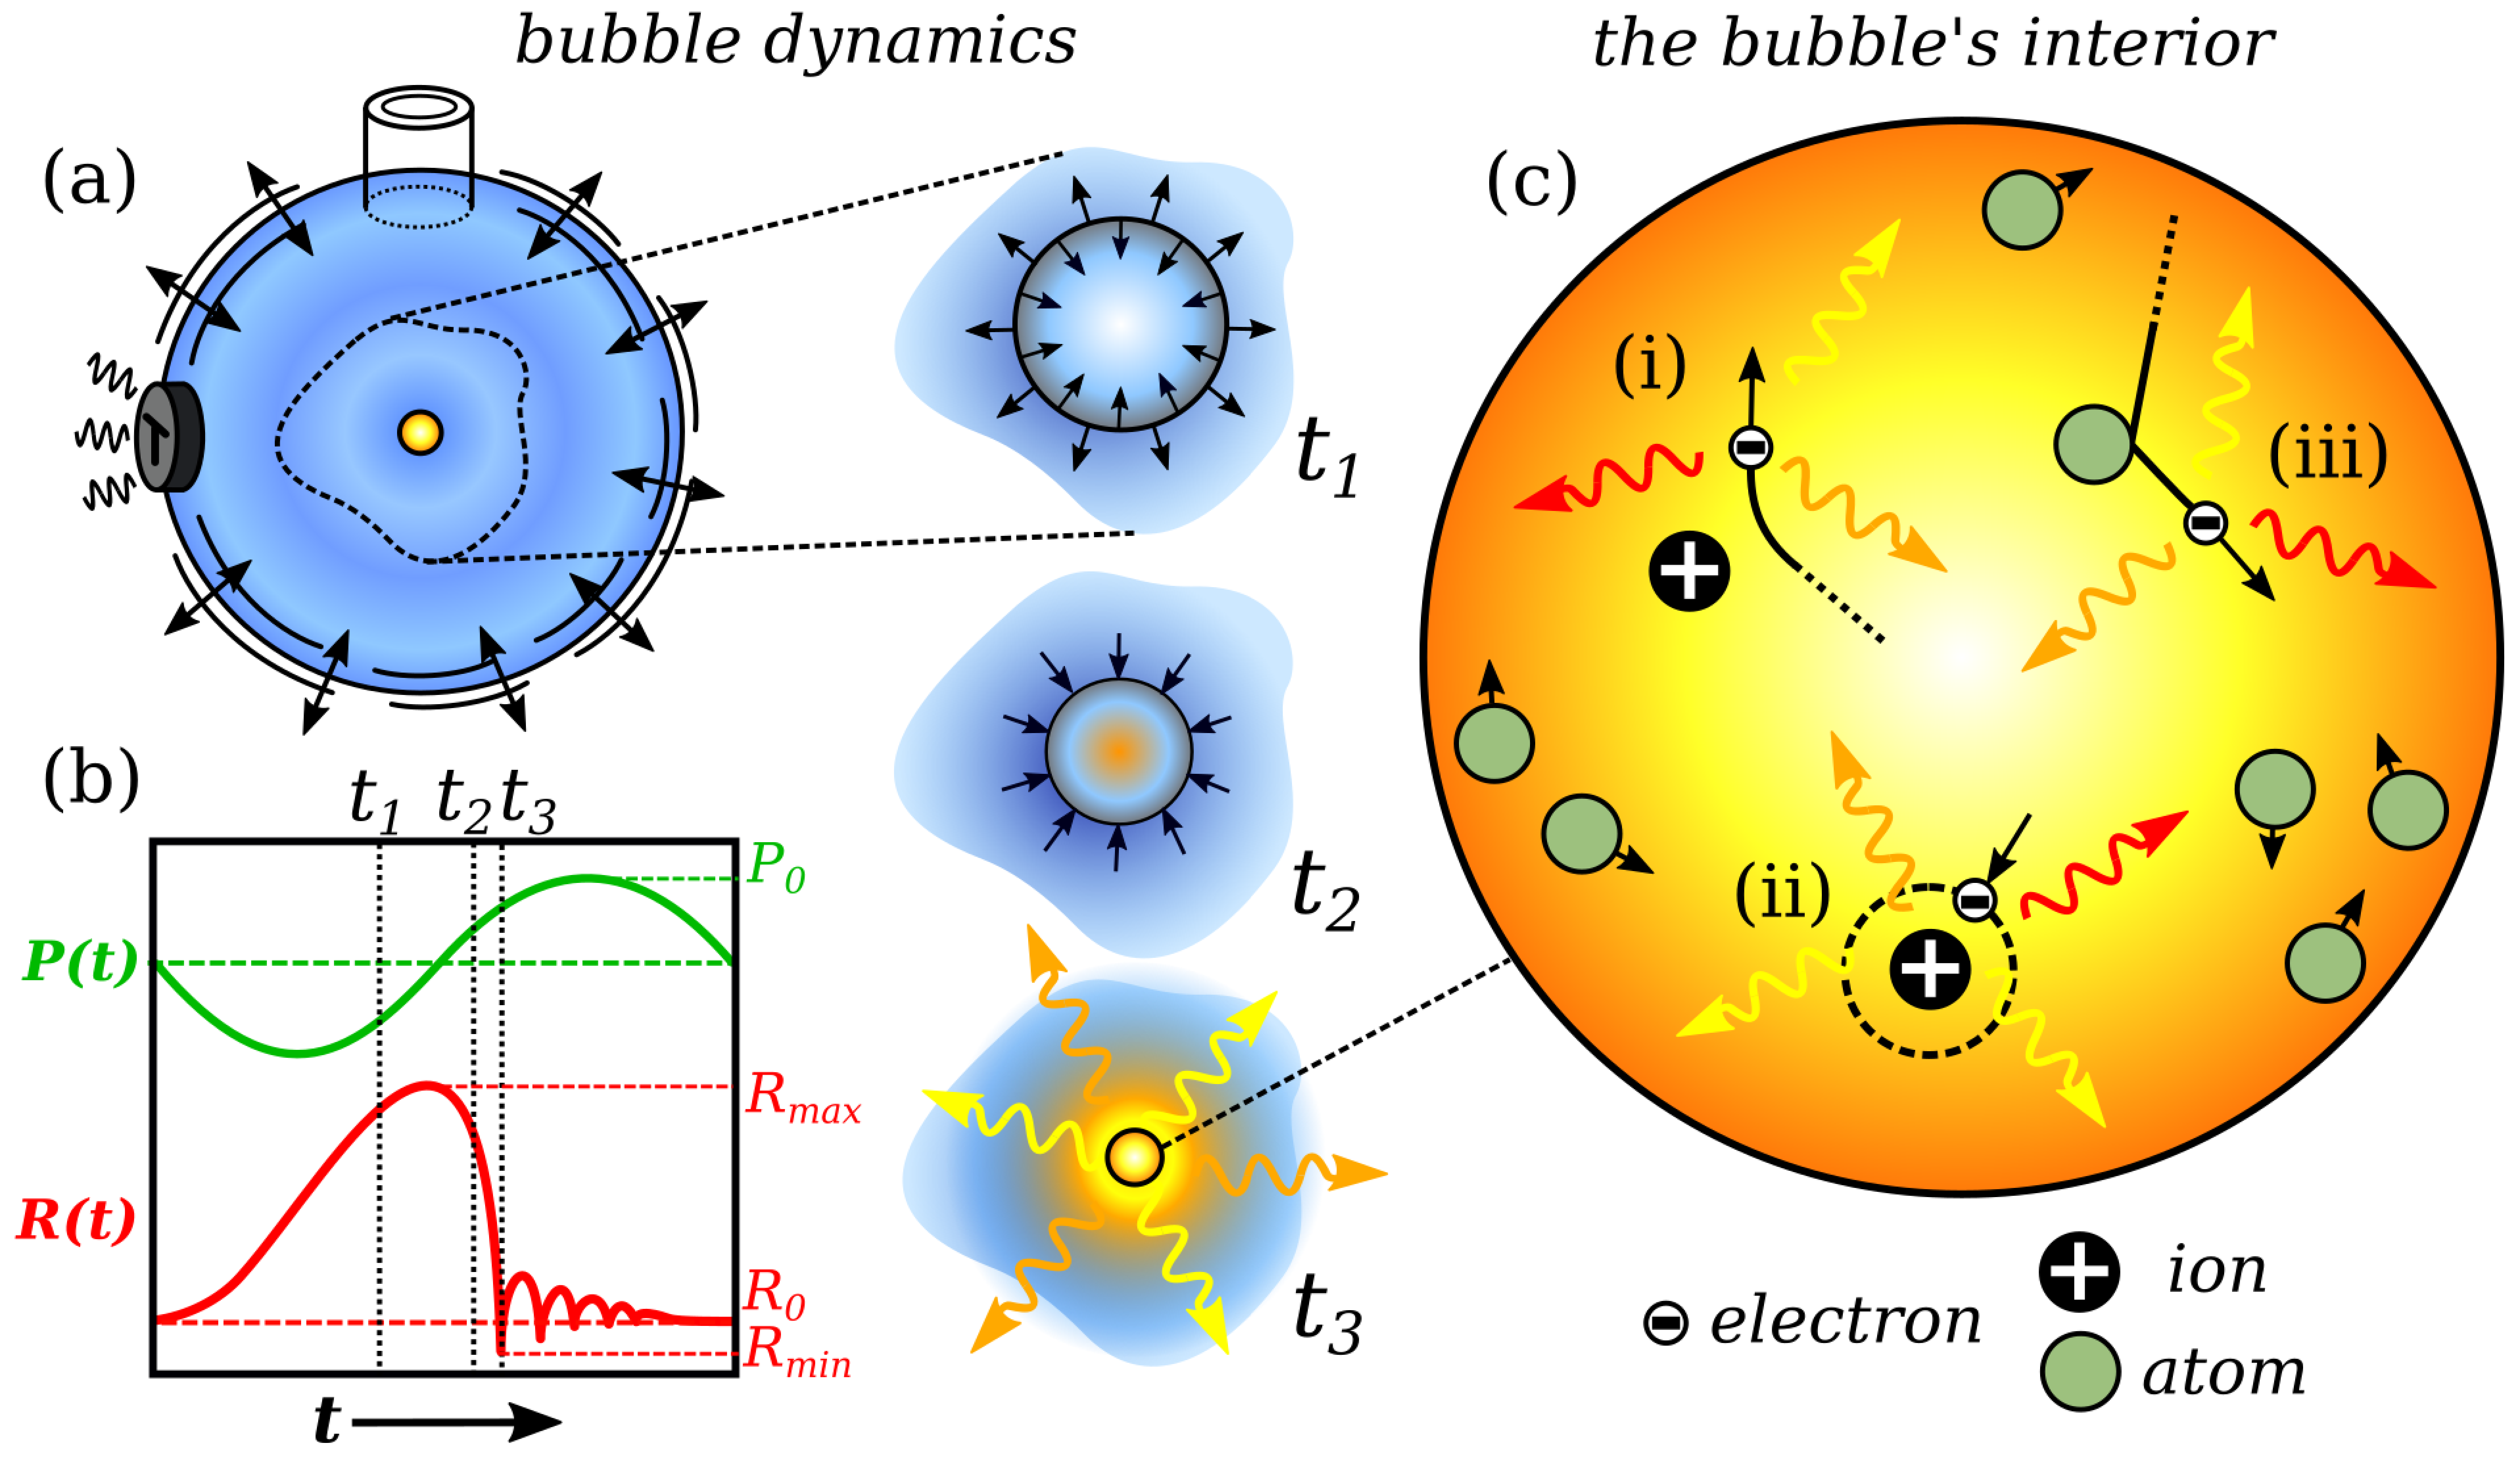
\includegraphics[width=0.9\linewidth]{figs/summary_fig}
    \caption{Schematic of the physics of SBSL. (a) Diagram of an SBSL experiment with a zoomed-in region around the bubble at different times shown to the right. A transducer, labeled as ``T", drives the flask and bubble. (b) Time-dependence of the driving pressure $P(t)$, bubble radius $R(t)$, and number of photons emitted $I(t)$, during SBSL. $P_0$ is the driving pressure amplitude, $R_0$ is the ``ambient" radius of the bubble, and $I_0$ is the peak number of photons emitted during the light pulse. (c) Inside the bubble during the light pulse at $t=t_3$. Electrons, ions, and atoms are labeled in the legend. The mechanisms of light emission are (i) electron-ion bremsstrahlung, (ii) electron-ion recombination, and (iii) electron-atom bremsstrahlung. }
\label{fig:summary_fig}
\end{figure}

The interior of the bubble is depicted at $t=t_3$ in Fig. \ref{fig:summary_fig} (c). When the temperature is $\sim 10,000$ K, about $1 \%$ of the atoms in the gas ionize \cite{hilgenfeldt1999simple,yasui1999mechanism}, creating pairs of free electrons and positively charged ions. When a free electron passes near an ion, it is accelerated by the Coulomb force. The electron's kinetic energy changes and the lost energy is converted into radiation \cite{zel2002physics,griffiths2005introduction,jackson1999classical}. This process is called \emph{electron-ion bremsstrahlung} (``bremsstrahlung" means ``braking-radiation") and is labeled as (i) in Fig. \ref{fig:summary_fig} (c). Similarly, if an electron and an ion combine to form a neutral atom, light is emitted as their energies change: \emph{electron-ion recombination} is labeled as (ii). 
The Coulomb force is long-ranged so even at low densities of electrons and ions, electron-ion bremsstrahlung is important \cite{zel2002physics}. Still, most of the particles are neutral atoms. Ordinarily, electron-atom scattering would be irrelevant since the electron-neutral particle interaction is very short-ranged. However, the pressure and density in the bubble at maximum compression are so large that electrons frequently collide with atoms, emitting radiation through \emph{electron-atom bremsstrahlung}. This mechanism is labeled as (iii) in Fig. \ref{fig:summary_fig} (c). Electron-ion bremsstrahlung, electron-atom bremsstrahlung, and electron-ion recombination are the most important mechanisms that produce light during SBSL \cite{hilgenfeldt1999simple,hilgenfeldt1999sonoluminescence,an2006mechanism,an2008spectral,an2009diagnosing,suslick2008inside}.

The goal of the rest of this paper is to present the theory needed to understand shrimpoluminescence in detail, though we will mainly focus on SBSL \footnote{It is apparently simpler to characterize SBSL without involving shrimp; convincing the shrimp to snap requires tickling them \cite{lohse2001snapping,versluis2000snapping,lohse2018bubble}. Besides notable exceptions \cite{tang2019bioinspired}, practically all work on SBSL has not involved shrimp.}. First, we will look at the problem of the fluid containing the bubble and derive the equations of motion for the bubble's wall. Next, we will use our results for the bubble's wall to understand the dynamics of the gas trapped in the bubble, calculating the temperature along the way. Finally, we will see how knowing the mechanisms of light emission/absorption in the bubble allow us to calculate the wave-length dependence of the bubble's light spectrum. Throughout the course of our journey, we will stick to the simplest results that still contain the essential physics we need. Connections to more advanced treatments, and their implications, are provided for completeness.

%MBSL was discovered by accident in 1933 when engineers trying to accelerate photo-development noticed that a photo-sensitive plate immersed in an ``insonated" fluid became foggy from exposure to light \cite{marinesco1933actions,frenzel1934luminescenz}. This wasn't ground-breaking since there was no practical use for the light emission and it was already known that cavitating bubbles, e.g. those generated by the sound field, could do tremendous damage to ship's propellers. The discovery's impact is summarized by Brenner: ``if the cloud [of cavitating bubbles] collapses violently enough to break molecular bonds in a solid, why should it \emph{not} emit photons" \cite{brenner2002single}. 

%Still, little information was accessible about the light emission until the 1990's when it was discovered that stable \footnote{\emph{Stable} is compared with \emph{transient} when discussing cavitation. A stable bubble persists through multiple cycles of cavitation, oscillating non-linearly around an equilibrium size. Transient bubbles appear and then collapse to disappear} single bubbles could be created and driven to emit light in SBSL \cite{gaitan1990experimental,gaitan1992sonoluminescence,crum1994sonoluminescence}. SBSL, unlike previous studies on MBSL, allowed very precise control and measurement of the SL process. Practically all progress on understanding SL has come from SBSL, with some authors even calling it ``the hydrogen atom of sonoluminescence" \cite{lohse2018bubble,crum1994sonoluminescence}. In SBSL, light emission from an isolated bubble is not complicated by scattering off other bubbles. Similarly, the bubble is not perturbed by interaction with other bubbles or, due to its tiny extent, by interaction with the container walls. Both theory and experiments are greatly simplified compared to MBSL. 

%SBSL still remained mysterious for some time, however. Measurements of the light spectrum from SBSL resulted in a nearly featureless continuum [Fig. \ref{fig:exp}, (bottom left)], leading to speculation that the light emission was very high-temperature thermal radiation \cite{hiller1992spectrum,hiller1994effect}. Around the same time, it was found that the light pulse was orders or magnitude shorter than the time in which the bubble was compressed to its smallest radius \cite{barber1992resolving,barber1991observation}. This discovery implied that SL was nearly decoupled from the bubble's dynamics and models were proposed based on \emph{converging shock waves} at the bubble's center with estimates of the temperature at $\sim10^8$ K \cite{wu1993shock,greenspan1993sonoluminescence}. These very high estimates for the temperature in the bubble finally led to a spark of interest more broadly: if the temperature were really that large, then it should be possible for nuclear \emph{fusion} to occur. An action movie featuring Keanu Reeves was made with this concept at the center of the plot \footnote{It is called \emph{Chain Reaction} and I am unwilling to watch it.} and in the early 2000's several papers were published claiming that nuclear fusion was possible in the lab using methods based on SBSL \cite{taleyarkhan2002evidence,taleyarkhan2004additional}. Unfortunately these studies turned out to be fraud \cite{reich2009bubble} and evidence eventually emerged that bubble distortions prevent converging shock-waves, severely reducing estimates for the temperature \cite{brenner2002single}. Current estimates for the temperature, which we will study in the rest of this paper, put the center of a sonoluminescing bubble between $10,000-30,000$ K \cite{flannigan2005plasma,flannigan2005plasma1,suslick2008inside,yasui2018acoustic,an2009diagnosing,an2008spectral,an2006mechanism}. 

\section{Bubble Dynamics}

 
Lord Rayleigh solved the problem of a vapor filled cavity collapsing in water (the so-called Rayleigh collapse), giving the first rigorous theoretical treatment of cavitation in the early 1900's \cite{rayleigh1917pressure,plesset1977bubble}. He found that the bubble wall's velocity diverges during collapse, giving rise to ``cavitation." Since then, the theory of \emph{bubble dynamics} has been refined considerably and we will devote a large portion of the paper to it \cite{prosperetti1999old,plesset1977bubble,plesset1977bubble,brenner2002single,lofstedt1995sonoluminescing,barber1992resolving}. We split this is split into parts. First, we derive the equations of motion for the bubble's wall. Then we review some important experimental developments that allow us to use a simple model for the dynamics of the gas in the bubble. Finally, we compare results of simulated bubble dynamics to experimental data. The connection to experiment is what allows us to calculate the temperature in real bubbles.

\subsection{The Bubble Wall}
It turns out the dynamics in SBSL are quite well described both qualitatively and quantitatively by the classical theory of bubble dynamics \cite{prosperetti1999old,brenner2002single,prosperetti1986bubble,plesset1977bubble,suslick2008inside,yasui2018acoustic,brennen2014cavitation}. The most widely known modern work is that of Plesset \cite{plesset1977bubble,plesset1949dynamics,prosperetti1986bubble}, resulting in the so called ``Rayleigh-Plesset" (RP) equation which we derive in this section. The field of bubble dynamics is quite mature and is too large to review here; instead, the reader is referred elsewhere \cite{prosperetti1999old,brenner2002single,prosperetti1986bubble,brennen2014cavitation}. 

We start with some assumptions. We assume the host liquid is incompressible, ultimately resulting in neglecting effects of sound radiated by the bubble. We also assume irrotational flow so that there is only radial motion in the liquid, i.e. $\bm{u}=u\bm{r}$ is the fluid's velocity with $u$ the speed and $\bm{r}$ the radial unit-vector. Then we can represent the velocity as the gradient of a scalar function: $u\bm{r}=(\partial_r \phi) \bm{r}$ \cite{jackson1999classical}. This amounts to assuming that the bubble is always spherical which seems like a rather drastic approximation but is validated experimentally \cite{prosperetti1999old,brenner2002single}.  %The fact that the bubble tends to remain spherical is understood by accounting for surface-tension at the liquid-bubble interface \cite{prosperetti1999old}.

Next, we assume that viscosity is negligible in the bulk dynamics of the liquid. In nearly incompressible, low-viscosity fluids such as water, this is a good approximation \cite{prosperetti1986bubble,prosperetti1999old,brenner2002single,plesset1977bubble}. We will account for viscosity later when looking at the bubble-liquid interface. Furthermore, since the bubble ($\sim\mu$m) is tiny compared to the flask ($\sim$ cm), we treat the dynamics of the liquid as if there is no bubble present. Similarly, we imagine the bubble is in an infinite, isotropic medium. The bubble-liquid interface enters both systems as a boundary condition later.

With these simplifying assumptions, the Navier-Stokes equation for momentum conservation in the fluid is \cite{prosperetti1999old,prosperetti1986bubble,leighton2007derivation,brennen2014cavitation}
\begin{equation}
\begin{split}
     \partial_r \left[ \partial_t \phi +\frac{1}{2} \left( \partial_r \phi \right)^2 \right] & = - \frac{1}{\rho} \partial_r p  \\ 
     %\partial_t \rho+ \partial_r \phi \partial_r \rho + \rho \partial^2_r \phi & = 0.
     \label{eq:NS_1D}
\end{split}
\end{equation}
We can integrate this using the fact that the compressibility is negligible \cite{leighton2007derivation}. On the left side, we take the velocity to vanish at infinity. On the right side, we assume that only the static and driving pressures, $p_\infty$ and $P(t)$ respectively, are relevant so that \cite{prosperetti1999old,prosperetti1986bubble,leighton2007derivation} 
\begin{equation}
    \partial_t \phi + \frac{1}{2}\left( \partial_r \phi \right)^2 = \frac{(p_\infty+P(t))-p(t,r)}{\rho}.
    \label{eq:press_vel}
\end{equation}

The velocity potential, $\phi$, approximately satisfies the wave equation $\nabla^2 \phi - (1/c^2)\partial_t^2 \phi =0 $ with $c$ the speed of sound in the fluid (this is exact in the limit $u/c\rightarrow 0$) \cite{leighton2007derivation,brenner2002single,prosperetti1999old}. We use incompressibility again by recalling that for an incompressible fluid $c\rightarrow \infty$. Then $\nabla^2 \phi =0$ and we can ignore retardation effects, writing the solution of $\nabla^2 \phi$ as $\phi = \psi(t)/r$ with $\psi$ a time-dependent coefficient \cite{prosperetti1999old,prosperetti1986bubble,leighton2007derivation}. The boundary condition for the velocity at the bubble wall, $u(R)\equiv \dot{R}$ with $R$ the bubble radius, gives $\psi= -R^2 \dot{R}$ and $\phi = -R^2 \dot{R}/r$. Plugging this into the left hand side of eq. \ref{eq:press_vel} and evaluating at the bubble wall, we arrive at the Rayleigh-Plesset equation \cite{prosperetti1999old,prosperetti1986bubble,leighton2007derivation,plesset1949dynamics,plesset1977bubble}
\begin{equation}
    R\ddot{R}+\frac{3}{2}\dot{R}^2 = \frac{p_B(t)-(p_\infty+P(t))}{\rho}
    \label{eq:RP_1}
\end{equation}
with $p_B \equiv p(r=R,t)$ the pressure in the fluid at the bubble wall. The combination $p_\infty+P(t)$ is the ambient pressure \cite{prosperetti1999old,prosperetti1986bubble} which gives the pressure in the absence of the bubble. The left hand side of eq. \ref{eq:RP_1} may be regarded as the kinetic energy (density). The right hand side is the change in enthalpy (density) due to the fluctuating bubble, i.e. the dynamics of the bubble given on the left hand side are determined by the enthalpy in the fluid due to the bubble's motion. In deriving this equation, we have assumed that the speed of propagation in the fluid is infinite. In reality, this is not true but this approximation will be very good close to the bubble (in the \emph{near-field}) where retardation effects are negligible anyway. In a similar way, we have assumed that the energy in the fluid due to distorting its volume is negligible. This approximation will be accurate near the bubble as well since the kinetic energy in this region will dominate \cite{prosperetti1999old}.

Eq. \ref{eq:RP_1} can be refined a little further. Since the motion in the fluid is purely radial, we expect the only relevant stresses to be normal to the bubble wall. Balancing these stresses at the bubble wall gives \cite{brenner2002single,leighton2007derivation,prosperetti1999old,prosperetti1986bubble}
\begin{equation}
    p_B(t)=p_g(t)-\frac{1}{R}\left( 2\sigma+4\eta \dot{R} \right)
    \label{eq:p_B}
\end{equation}
with $p_g(t)$ the pressure in the gas at the bubble wall. The term $\sim\sigma$ is called the \emph{Laplace pressure} and is from surface tension at the bubble-liquid interface. The $\sim\eta$ term is due to the \emph{bulk viscosity} in the fluid. The surface tension and viscosity coefficients, $\sigma$ and $\eta$ respectively, are assumed known. The RP equation becomes
\begin{equation}
    R\ddot{R}+\frac{3}{2}\dot{R}^2 = \frac{1}{\rho} \left[ p_g(t)-p_\infty-\frac{1}{R}\left( 2\sigma+4\eta \dot{R} \right)-P(t) \right]
    \label{eq:RP_2}
\end{equation}
With the above assumption that the compression is adiabatic, the conditions inside the bubble are decoupled from the liquid (besides the coupling through the RP equation) and we temporarily consider $p_g(t)$ to be a known quantity. $P(t)$, the time-dependent part of the pressure in the absence of the bubble, is from an external source. In SBSL, the sources are the transducers driving the flask and $P(t)$ is an acoustic plane wave. Keller and coworkers showed that the modification required to the RP equation is the replacement $P(t) \rightarrow P_0 \sin(\omega t)$ \cite{keller1980bubble}. $P_0$ is the driving pressure amplitude and $\omega$ is the driving frequency.

%\begin{figure}
%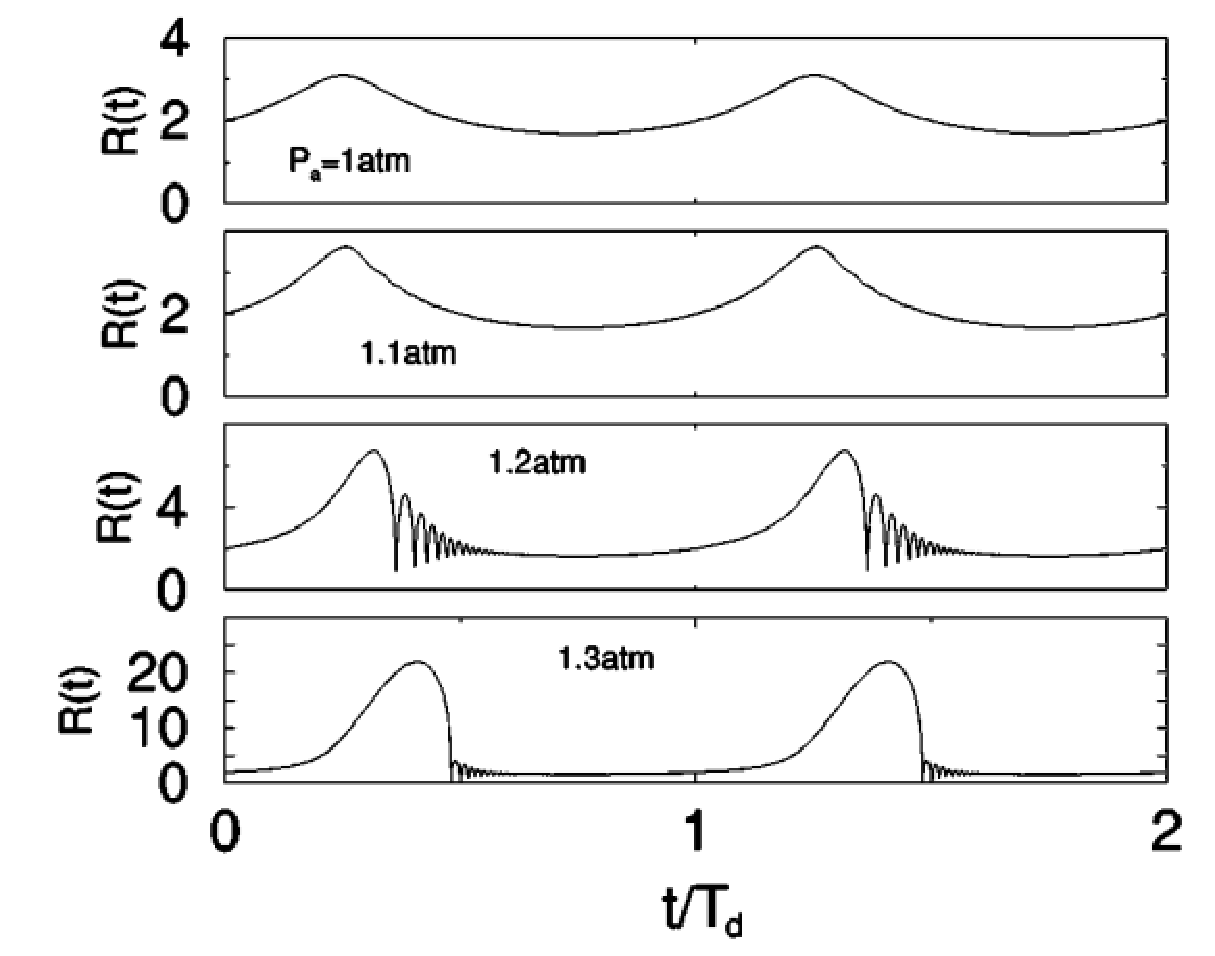
\includegraphics[width=0.5\linewidth]{figs/bubble_radius_2.pdf}
%    \caption{Solutions to eq. \ref{eq:RP_2} for different driving pressures. For driving at 1 atm, the dynamics are a simple pulsating bubble. For larger driving pressure, e.g. 1.2 atm, we observe strongly non-linear behavior exhibiting cavitation and afterbounces. For even larger driving pressure, we encounter the regime where SBSL begins to occur. From ref. \cite{brenner2002single}}
%\label{fig:bubble_radius_2}
%\end{figure}

The RP equation (eq. \ref{eq:RP_2}) is pretty but its analytical solution is intractable. Direct solutions of the RP equation or its variants are done numerically using Euler or Runge-Kutta methods \cite{yasui2018acoustic,yasui2015dynamics}. It is no great challenge computationally. For now, let's see what we can understand analytically by making some more approximations. We look at the interval where the bubble wall's velocity is very large, called \emph{the Rayleigh collapse}. Here, the right hand side of eq. \ref{eq:RP_2} will be much smaller than the $\dot{R}^2$ term and we may neglect it \cite{rayleigh1917pressure,plesset1949dynamics,prosperetti1999old,brenner2002single}. Rayleigh looked at the same problem:
\begin{equation}
    \ddot{R}=-\frac{3}{2} \frac{\dot{R}^2}{R}.
    \label{eq:Rayleigh}
\end{equation}
The right hand side of eq. \ref{eq:Rayleigh} is always positive, so the acceleration is always negative. The bubble wall's \emph{speed} gets larger, causing larger negative acceleration, which increases the speed... in this way, the bubble collapses. Eq. \ref{eq:Rayleigh} can be solved and the result is $R(t)\sim\left(1-t/\tau \right)^{2/5}$, with $\tau$ satisfying $R(\tau)=0$; the velocity, $\dot{R}\sim\left(1-t / \tau \right)^{-3/5}$, diverges. These observations are what lead to Rayleigh's argument for the origin of cavitation damage to ship's propellers. %Yasui gave a rather elegant heuristic explanation for the origin of \emph{cavitation} in a fluid that is worth stating here \cite{yasui2018acoustic}. Consider the mass flowing through concentric shells around a bubble, $4\pi R_i^2 v_i \rho$. For a source free field, we require that neighboring shells satisfy conservation of mass: $4\pi R_1^2 v_1 = 4\pi R_2^2 v_2$. For $R_2 > R_1$, we see that $v_1/v_2 = \left(R_2/R_1\right)^2$. The velocity for a smaller radius is always larger, diverging towards the origin.

In reality, the bubble's velocity is always finite and in the case of \emph{stable} SBSL, so is the radius. In the full RP equation (eq. \ref{eq:RP_1}) the only term capable of compensating the bubble wall's motion is the diverging pressure inside the bubble \cite{brenner2002single}. If we had not assumed incompressibility, eq. \ref{eq:RP_1} would also include terms from the sound radiated by the bubble. A family of solutions, collectively called ``Rayleigh-Plesset equations," are derived in this way \cite{prosperetti1986bubble,prosperetti1988nonlinear,keller1956damping,lezzi1987bubble}. It turns out that the most important term for slowing the bubble wall's diverging velocity is $\propto\dot{p}_g$. Keeping only this term results in another popular variant of the RP equation that is only slightly more complicated than eq. \ref{eq:RP_2} \cite{lofstedt1995sonoluminescing,barber1997defining}. The observed error between this equation and experiment is only significant shortly after the Rayleigh collapse and it is quantitatively in good agreement with measurements of the bubble's radius during the rest of the cycle \cite{brenner2002single}. 

Above, we assumed that the bubble always remains spherical. Of course this isn't always true and \emph{shape-instabilities} occur for the right combinations of mechanical properties and driving force/frequency. Usually shape-instabilities destroy the bubble and kill SBSL so we won't focus on these issues here. We will always assume we are in a parameter-regime where SBSL occurs. The reader is referred to one of several reviews on the \emph{phase-space} of SBSL for details \cite{yasui2018acoustic,brenner2002single,hilgenfeldt1999sonoluminescence,an2009diagnosing}. 


\subsection{The Bubble's Interior}
Progress on understanding the bubble's \emph{interior} since the discovery of SBSL in the 1990's \cite{gaitan1992sonoluminescence} follows two paths \cite{brenner2002single,suslick2008inside,yasui2018acoustic}: (i) model calculations based on the RP equations and an equation of state for the pressure (from which we may calculate the temperature) are used to try to reproduce the easily measurable dynamics of the bubble. (ii) We model the light emission itself and compare our calculation to spectroscopic measurements of SBSL \cite{hiller1992spectrum,brenner2002single}. 
%Obviously these are related topics, but the distinction in the context of SBSL is important as we will now see.

Most early progress on the bubble's interior depended on the former method: if we predict the right dynamics, then we might know the correct pressure and temperature in the bubble. These data are then used to try to describe the light emission. Calculating the dynamics of the bubble's wall from one of the RP equations (e.g. eq. \ref{eq:RP_2}) requires the pressure inside the bubble as input. We need a suitable form for $p_g(t)$ in the RP equations that reproduces the measured radius-time curve $R(t)$ for a stable cavitating bubble. It turns out that this is a very complicated problem: gas diffusion between the bubble and liquid varies the number of particles present and, to make things worse, the conditions inside the bubble facilitate chemical reactions between the air and water-vapor, changing the properties of gas dynamically \cite{brenner2002single}. Brenner et. al elegantly summarized the significance of this problem \cite{brenner2002single}: ``one of the exciting features of modern research on SBSL is that it is a testing ground for how well mathematical models can deal with such a complicated situation."

\begin{figure}
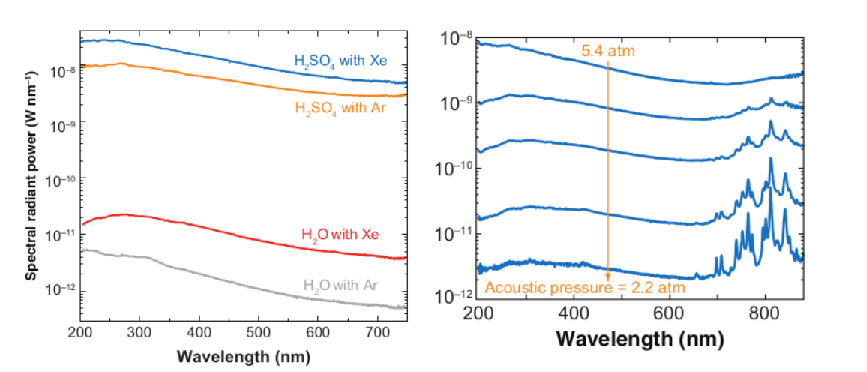
\includegraphics[width=0.9\linewidth]{figs/exp.pdf}
    \caption{(left) Emission spectra as a function of wave-length, $\lambda$, for Ar and Xe bubbles in water and 85\% aqueous H$_2$SO$_4$. The pressure was optimized to give maximum intensity of emitted light. (right) Emission spectra as a function of wave-length, $\lambda$, for an Ar bubble in 85\% aqueous H$_2$SO$_4$ at different driving pressures, $P_0$. The spectral lines around $\sim 800$ nm are from Ar $4s\leftrightarrow4p$ transitions and disappear with increasing driving pressure. From ref. \cite{suslick2008inside}}
\label{fig:exp}
\end{figure}

The other way to understand the bubble's interior is its light spectrum. For the first decade or so, SBSL experiments were mainly done with \emph{air} bubbles in water \cite{suslick2008inside,brenner2002single,gaitan1992sonoluminescence}. Careful measurements of light emission from SBSL in water resulted in an almost featureless spectrum (see Fig. \ref{fig:exp}) and attempts to fit it as black-body radiation were not successful \cite{hiller1992spectrum}. Little progress was made on this front for quite some time \cite{brenner2002single}. The utility of analyzing the light spectrum of SBSL in water is succinctly described by Suslick \cite{suslick2008inside}: ``because of the inherent ambiguity associated with the analysis of featureless spectra of unknown origin, a more rigorous explanation [of SBSL] is unlikely to be generated". 

Some attempts were made to measure SBSL using non-aqueous liquids (e.g. alcohol, silicone oil) but experiments were not very successful \cite{weninger1995sonoluminescence,barber1997defining,barber1997defining}. Eventually, different gases were tried in water. Air is $\sim 80\%$ N$_2$, $\sim 20\%$ O$_2$, and $\sim 1\% $ Ar so, naturally, pure O$_2$ or N$_2$ were tried first. Degassed water \emph{regassed} with N$_2$, O$_2$, or even a mixture of O$_2$ and N$_2$ did not to produce SBSL \cite{hiller1994effect}. It was discovered that a noble-gas was required for SBSL to occur \cite{barber1997defining,hiller1994effect,brenner2002single}. This resulted in the \emph{argon rectification hypothesis}, which claims that all species in the air inside the bubble besides Ar are gradually ejected until all that remains is pure Ar \cite{lohse1997sonoluminescing,brenner2002single,yasui2018acoustic,suslick2008inside}. The hypothesis is based on the fact that, at the high temperature inside the bubble, dissociation of O$_2$ and N$_2$ is possible. These species react with dissociated water vapor radicals to form new species that are soluble in water. As the pressure becomes very large during the compression stage of SBSL, the soluble materials leave the bubble and do not re-enter since their solubility in water is enormous compared to the Ar content of the bubble \cite{lohse1997sonoluminescing}. Over many cycles, the contents of an air bubble in water become nearly pure Ar. It was also realized that SL would be much more intense if the contents of the bubble are a pure inert gas: if the contents are e.g. molecules, the specific heat of the gas is larger, resulting in lower temperature and decreased light production from the bubble \cite{brenner2002single,yasui2018acoustic,lohse2018bubble,suslick2008inside}. This mechanism is used to explain the relatively weak light observed in MBSL: the bubbles are transient and cannot eject a significant amount of O$_2$ or N$_2$ over a single cycle. The current belief is that the contents of a bubble undergoing SBSL in water are (nearly) pure Ar after $\sim 10^3$ cycles \cite{brenner2002single,yasui2018acoustic}.  

Most studies continued to use water as the host liquid until it was realized that SBSL in aqueous H$_2$SO$_4$ produces light $10^3$ times brighter than in water, allowing more precise measurements of the light spectrum \cite{flannigan2005plasma,flannigan2005plasma1,flannigan2006measurement}. The mechanical properties in aqueous H$_2$SO$_4$ allow stable SBSL with larger bubble radii than in water, increasing the emitting volume. More importantly, new measurements revealed the phase space of SBSL in aqueous H$_2$SO$_4$ included a much larger range of driving pressure than water [Fig. \ref{fig:exp} (right)]. SBSL in aqueous H$_2$SO$_4$ could be driven at very low pressure, leading to much lower temperature bubbles, while driving at large pressure led to conditions similar to SBSL in water. 

Careful experiments revealed that the spectrum depended critically on the noble-gas content and driving pressure. Suslick et. al measured the emission spectra from Ar, Xe, and Kr bubbles in aqueous H$_2$SO$_4$ \cite{flannigan2005plasma,flannigan2005plasma1,flannigan2006measurement,suslick2008inside}. At low driving pressure, they identified spectral lines from Ar$^+$, Xe$^+$, and Kr$^+$ excited state transitions, proving that the core of the bubble is plasma. Perhaps equally as crucially, they found the absence of emission lines from components of aqueous H$_2$SO$_4$ vapor at large driving pressure \cite{suslick2008inside,flannigan2006measurement,flannigan2006measurement}: the plasma contained only the noble-gas, experimentally confirming the argon rectification hypothesis. This work also explained why the spectrum in water is featureless; the large pressure in SBSL in water results in an increased collision rate between particles, broadening the spectral lines until they are no longer visible  \cite{an2009diagnosing,suslick2008inside,flannigan2005plasma,flannigan2005plasma1,flannigan2006measurement}.

The argon rectification hypothesis greatly helped to refine models for the gas dynamics in the bubbles and confirmed why simple models usually work well \cite{suslick2008inside,brenner2002single}. With this in mind, we will only focus on a simple model for the gas dynamics in this paper. Modern reviews on modelling the bubble's interior in SBSL exist elsewhere \cite{brenner2002single,yasui2018acoustic,brennen2014cavitation}. 

\subsection{Gas Dynamics}
The most straightforward way to model the gas dynamics in the bubble is through direct solution of the Navier-Stokes equations for the gas \cite{brenner2002single}. In fact, the most accurate quantitative predictions of the conditions of the bubble's interior take this path \cite{an2006mechanism,an2008spectral,an2009diagnosing,flannigan2005plasma,flannigan2005plasma1,flannigan2006measurement}. Equations of motion with varying degrees of sophistication are derived and the coupled system of gas dynamical and RP equations are solved numerically. The discussion proceeds in much the same way as deriving the RP equations above but is considerably more complicated since we have to account for mass and heat transfer across the bubble wall \cite{brenner2002single,yasui2018acoustic}. Instead, we will look at a simple model and discuss how it can be extended to more accurately represent the dynamics.

Recalling that the bubble is (almost) purely noble-gas, a simple but reasonable model for the gas dynamics, at least during the collapse, is that of an adiabatically, quasistatically compressed Van der Waals gas \cite{brenner2002single,lofstedt1995sonoluminescing,barber1997defining,lofstedt1993toward,hilgenfeldt1999simple}. In the context of SBSL, the interaction term in the Van der Waals (VdW) equation of state is usually neglected and the only modification to the ideal gas result is the excluded volume of the real gas molecules, $V_h = 4 \pi h^3/3$, with $h$ the VdW \emph{hard-core radius}. The pressure in an adiabatically compressed \emph{ideal} gas at volume $V_2$ is \cite{schroeder1999introduction}
\begin{equation}
    P_2 = P_1 \left(\frac{V_1}{V_2}\right)^\gamma
\label{eq:P}
\end{equation}
where $P_1$ is the initial pressure at volume $V_1$ and $\gamma=C_P/C_V$ is the ratio of the constant-pressure and constant-volume specific heats respectively. In our case, we assume that our bubble has an ambient radius, $R_0$, where the pressure is at its equilibrium value, $p_0$. The ambient volume of the bubble is $V_0 =  4 \pi R_0^3/3$. It follows from our discussion of the RP equation that $p_0=p_\infty+2\sigma /R_0$. We want to calculate the pressure in the gas, $p_g(t)$, as a function of the bubble's radius, $R(t)$, determined from the RP equation. Plugging these data into eq. \ref{eq:P}, and subtracting the excluded volume, we arrive at a very commonly used equation in the context of SBSL \cite{brenner2002single,lofstedt1995sonoluminescing,barber1997defining,lofstedt1993toward,hilgenfeldt1999simple,sivasubramanian2002temperature}:
\begin{equation}
    p_g(t) = \left( p_\infty+2\frac{\sigma}{R_0} \right) \left[ \frac{R_0^3-h^3}{R^3(t)-h^3} \right] ^ \gamma
    \label{eq:p_g}
\end{equation}
It's clear that the purpose of the excluded volume is to make sure that if the bubble collapses so strongly that its contents become incompressible (i.e. $R(t)\rightarrow h$), the pressure diverges \cite{lofstedt1993toward,brenner2002single}.

Physical intuition tells us why eq. \ref{eq:p_g} is sensible during the bubble's collapse: the bubble wall's velocity is fast and very little heat can flow out during compression. During the expansion and after-bounce stages of the bubble's cycle, which comprise its majority, the gas dynamics should instead be regarded as \emph{isothermal} \cite{brenner2002single}. This is true because, when the bubble's velocity is comparable to the heat diffusion timescale, the temperature throughout the bubble is nearly equal to that in the liquid \cite{prosperetti1999old,brenner2002single,yasui2018acoustic}. The relevant modification to eq. \ref{eq:p_g} is replacing $\gamma\rightarrow 1$. A neat way of including both isothermal and adiabatic gas dynamics is continuously varying the exponent, $\gamma$ in eq. \ref{eq:p_g}, between its adiabatic and isothermal values, $C_P/C_V$ and $1$, respectively. This technique has been commonly used in calculations of SBSL in water \cite{hilgenfeldt1999simple,hilgenfeldt1999sonoluminescence,prosperetti1986bubble,brenner2002single}. Simple forms, e.g. eq. \ref{eq:p_g} with the constant adiabatic exponent $\gamma=5/3$, give close to the correct bubble dynamics with the most obvious error occurring during the isothermal after-bounces (see Fig. \ref{fig:mie}). 

%more advanced solutions of the gas Navier-Stokes equations improving only on estimates for the conditions inside the bubble \cite{brenner2002single,yasui2018acoustic}.

Recalling that one of main goals of modeling the bubble dynamics in SBSL was to calculate the temperature inside the bubble, we can also derive an equation for $T(t)$ \cite{barber1997defining,brenner2002single,sivasubramanian2002temperature}:
\begin{equation}
    T(t) = T_0 \left( \frac{R_0^3-h^3}{R^3(t)-h^3} \right)^ {\gamma-1}
    \label{eq:T(t)}
\end{equation}
We said that for most of the bubble's cycle, the gas dynamics is isothermal: $T_0$ is the temperature of the liquid. The only ``unknown" quantity still preventing us from simulating the bubble's dynamics and calculating the temperature is $R_0$ in eqs. \ref{eq:p_g} and \ref{eq:T(t)}. We learn how to determine $R_0$ in the next section.

\subsection{Bubbles in the Lab}

%\begin{figure}
%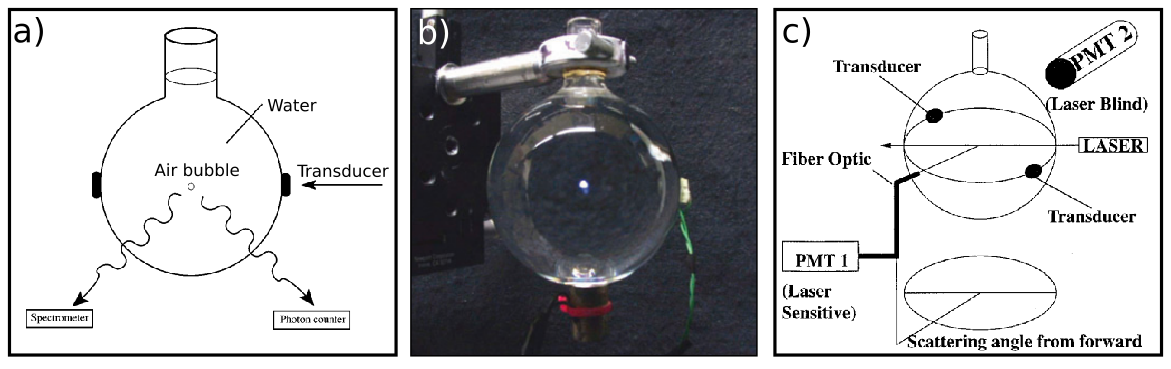
\includegraphics[width=0.9\linewidth]{figs/flask.pdf}
%    \caption{(a) Schematic of a spherical ``acoustic levitation cell". The piezoelectric transducers that drive the bubble trapped in the flask are labeled in the diagram. (b) Photograph of a sonoluminescing bubble in 85\% aqueous H$_2$SO$_4$. (c) Schematic of a Mie scattering experiment. Panels (a), (b), and (c) are from refs. \cite{brenner2002single}, \cite{suslick2008inside}, and \cite{gompf2000mie} respectively.}
%\label{fig:flask}
%\end{figure}

Creating stable, single bubbles in an experiment is not particularly challenging and can be done with standard and low-cost materials. A typical experimental setup is shown in Fig. \ref{fig:summary_fig} (a). Since we are concerned with explaining the light emission process itself, we will only sketch the experimental setup; it can be summarized as follows \cite{lentz1995mie,gaitan1990experimental,gaitan1992sonoluminescence,gompf2000mie,brenner2002single,yasui2018acoustic,brennen2014cavitation,suslick2008inside}. A suitable sample of liquid is placed into a flask. Stuck to the outside are piezoelectric transducers driven sinusoidally to excite a resonance of the flask: a typical flask is a few cm across with a resonance at $\approx 20$ kHz \cite{brenner2002single}. The frequency is chosen to form a pressure \emph{antinode} at the center of the flask, trapping a bubble there.

%Let us take a brief aside: in deriving the RP equations, we assumed the center of the bubble was stationary. Actually, this is what we want in an SBSL experiment and it is worth discussing under what conditions this is true. In an ideal, incompressible fluid the net force acting on a bubble may be written as 
%\begin{equation}
%    \bm{f}=-\int_{\partial \Omega} p \bm{n} dA = -\int_\Omega \nabla p dV
%\end{equation}
%Here, $\bm{f}$ is the net force, $p$ is the pressure at the bubble's surface, $\bm{n}$ is the unit normal vector point out of the bubbles surface, and $\partial \Omega$ is the bubble's boundary with $\Omega$ the bubble's domain. The last term is due to an application of Gauss's theorem. Bjerknes \cite{bjerknes1909kraftfelder} took $\nabla p \equiv \nabla p(r=0,t)$ to be constant and averaged over one period of oscillation to find 
%\begin{equation}
%    \bm{f} = -\frac{4}{3}\pi \langle R^3 \nabla p \rangle.
%    \label{eq:Bj_force}
%\end{equation}
%This is the so called \emph{Bjerknes force}. The point is that if the bubble is located at a pressure extrema, e.g. the antinode at the center of the flask, then this force should vanish and the bubble will remain stationary, an essential result for SBSL experiments.

%Some authors have looked at corrections to the bubble's dynamics in the presence of buoyancy, which cause translational motion even for vanishing Bjerknes force. The result is the bubble oscillates around an equilibrium position near but away from the center of the flask \cite{matula2000single,matula1997bjerknes,matula1999inertial}. The translational motion of the bubble leads to shape distortion which is believed to suppress SL; this is confirmed by SBSL experiments in microgravity resulting in larger intensity light production \cite{matula2000single}.

The driving pressures relevant to SBSL ($\sim 1.1-1.5$ atm) are too small to cause bubbles to form spontaneously \cite{brenner2002single}. Instead, a bubble is usually \emph{seeded} somehow. In the original work of Gaitan, an air bubble was injected using a syringe \cite{gaitan1992sonoluminescence}. More recently, seeding methods involve shooting a small jet of water into the flask (like our shrimp friends!) or blasting the water with a laser to boil a small volume \cite{suslick2008inside,yasui2018acoustic}. The later method is preferred as it enables more precise experimental control over the bubble's ambient radius, $R_0$.

Now let's discuss two experimentally accessible quantities that have turned out the be important. (i) The bubble's radius may be measured by \emph{Mie scattering} and compared directly to solutions of the RP equations, allowing us to ``measure" $T(t)$. (ii) The light can be analyzed with a spectrometer, giving us information on the bubble's contents: in principle, we can learn about temperature and pressure inside the bubble \cite{hiller1992spectrum,hilgenfeldt1999simple,flannigan2005plasma,flannigan2005plasma1,flannigan2006measurement}. We look at this in the next section.

\begin{figure}
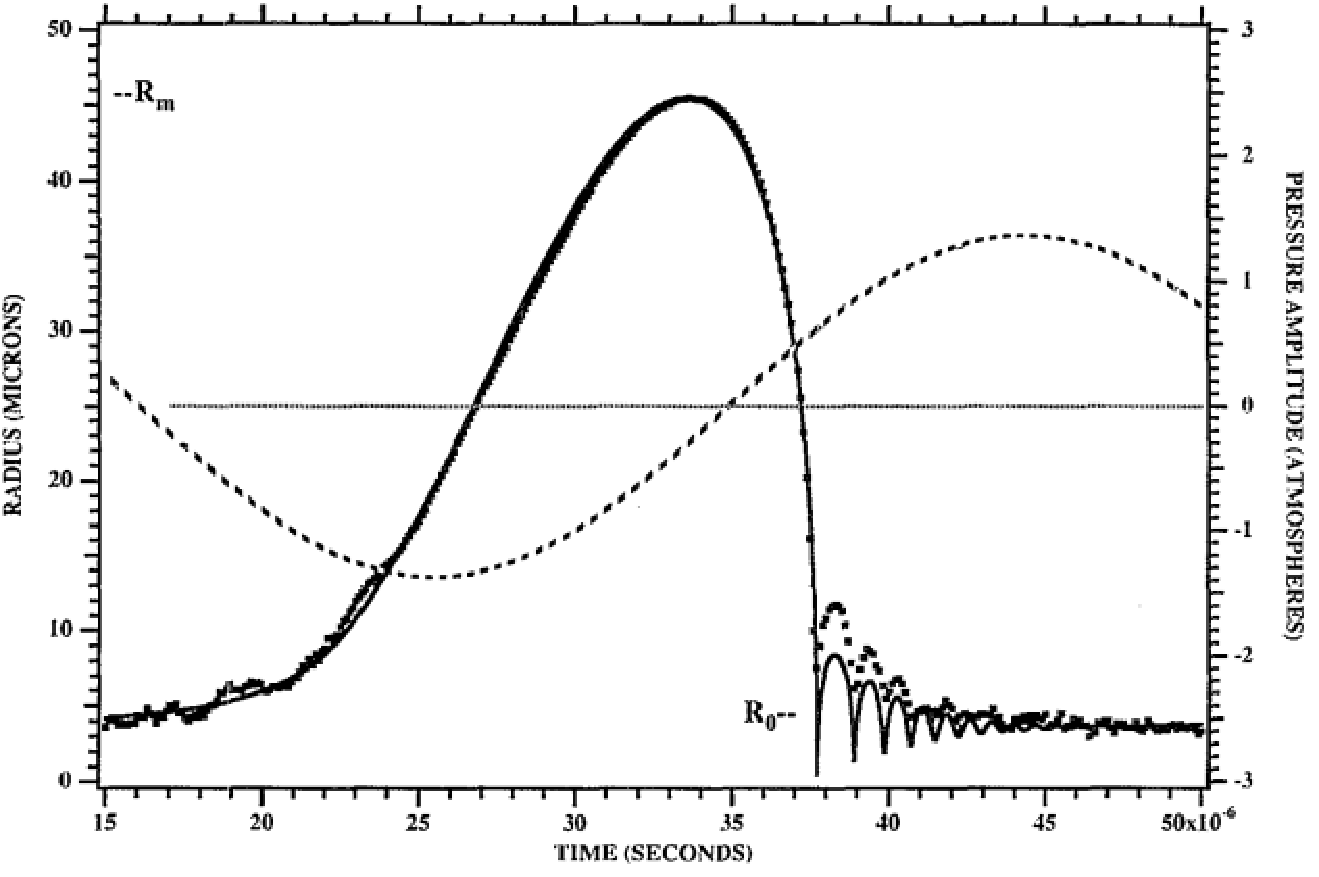
\includegraphics[width=0.6\linewidth]{figs/mie.pdf}
    \caption{Numerical solution of the $\propto \dot{p}_g$ RP equation variant discussed earlier with the gas dynamics given by the simple form in eq. \ref{eq:p_g}. The dots are experimental results from Mie scattering. The fit resulted in $R_0=4.5$ $\mu m$ and max temperature $8,500$ K. From ref. \cite{lofstedt1993toward}.}
\label{fig:mie}
\end{figure}

In Mie scattering, a laser is shot at a bubble and the scattered intensity is analyzed to determine $R(t)$ \cite{matula1999inertial,lentz1995mie}. Modeling the bubble as a homogeneous dielectric sphere \cite{jackson1999classical}, the angular distribution of light scattered from the bubble at \emph{fixed radius} and the time-dependent scattering off the bubble at \emph{fixed angle} allow use to accurately measure the bubble's radius as a function of time \cite{brenner2002single}. Results from a Mie scattering experiment are shown as dots in Fig. \ref{fig:mie}. Parameters used to calculate the gas dynamics in the bubble are fit to the measured radius to build a full model of the bubble dynamics. For the gas model in the last section, eq. \ref{eq:p_g}, the parameter to fit is $R_0$. Once we fit it, we know the temperature in the bubble from eq. \ref{eq:T(t)}. For the calculation in Fig. \ref{fig:mie}, the dynamics fit the experiment well, giving $R_0=4.5~ \mu$m and putting the ``measured" temperature at $8,500$ K. 

Before discussing the light spectrum, we note that it is possible to calculate the temperature from ``first-principles" without fitting to experiment. This can done by direct numerical solution of the gas's Navier-Stokes equations. The results are qualitatively similar to simple model calculations, but are in slightly better quantitative agreement when used to calculate the light spectrum \cite{an2009diagnosing,an2008spectral,an2006mechanism}. 

\section{Let there be light!}

Now that we know the temperature in the bubble, $T(t)$, we are finally ready to discuss the light emission. A requirement for models of light emission in SBSL is \emph{local thermodynamic equilibrium} (LTE). LTE is expected to be true in a bubble undergoing SBSL since the particle density ($\sim 10^{28}/m^3$) and temperature ($\sim 10^4$ K) are very large, causing collisions between particles to occur so frequently that equilibrium is guaranteed \cite{brenner2002single,hilgenfeldt1999sonoluminescence,yasui1999mechanism}. 

Any ordinary matter at finite temperature will continuously and spontaneously emit radiation. In LTE, the rate energy is emitted equals the rate it is absorbed \cite{zel2002physics}. This means that we only need to know \emph{either} the emission coefficient \emph{or} the absorption coefficient of a material to know the intensity that it emits radiation. The intensity, $I(\lambda,T)$, is the amount of energy passing per unit-time and unit-solid angle through a unit-area oriented perpendicular to the light's propagation direction. An ideal emitter/absorber is called a ``black-body."  For a black-body, the intensity is given by Planck's law: \cite{schroeder1999introduction}
\begin{equation}
    I_{B}(\lambda,T(t))=\frac{2 h c^2}{\lambda^5}\left[\exp\left(\frac{hc}{\lambda k_B T(t)}\right)-1\right]^{-1}
\end{equation}
The subscript $B$ is to remind us this is for a black-body. $\lambda$ is the wave-length of the light, $c$ is the speed of light in vacuum (we assume the index of refraction is $n\approx 1$ \cite{hilgenfeldt1999simple,hilgenfeldt1999sonoluminescence,zel2002physics}), $h$ is Planck's constant, and $k_B$ is Boltzmann's constant. We can use the temperature, $T(t)$, from eq. \ref{eq:T(t)}, to calculate the instantaneous intensity radiated in the bubble. Integrating over the bubble's volume and over time, we can calculate the number of photons produced during SBSL; a quantity that can be directly compared to experiment \cite{hilgenfeldt1999simple,hilgenfeldt1999sonoluminescence,an2006mechanism,an2008spectral,an2009diagnosing}. Calculations that assume the bubble is a black-body over-estimate the number of photons by orders of magnitude \cite{hilgenfeldt1999simple,brenner2002single}. We need to use a model that includes finite opacity.

Let's call the wave-length and temperature dependent absorption coefficient $\kappa(\lambda,T)$. For a ray of light emitted somewhere in the bubble, the intensity after travelling a distance $s$ is \cite{zel2002physics,hilgenfeldt1999simple,taylor1969experimental}
\begin{equation}
    I(\lambda,T(t))=I_{B}(\lambda,T(t))  \left[ 1-\exp \left( -\kappa[\lambda,T(t)] s \right) \right].
    \label{eq:intensity}
\end{equation}
We are assuming that that the temperature in the bubble is spatially uniform so that $\kappa$ is too \cite{hilgenfeldt1999sonoluminescence,hilgenfeldt1999simple}. In the limit that $\kappa \rightarrow\infty$, i.e. an opaque bubble, we recover the result for a black-body emitter. On the other hand, for a nearly transparent bubble, $\kappa \ll 1$ and $I\approx I_B \kappa s$. The number of photons emitted is greatly reduced; a result that what we require. A great deal of work has been devoted to identifying the relevant absorption mechanisms leading to $\kappa(\lambda,T)$ \cite{hilgenfeldt1999simple,brenner2002single,hilgenfeldt1999sonoluminescence,yasui1999mechanism,flannigan2005plasma,flannigan2005plasma1,flannigan2006measurement,suslick2008inside,an2009diagnosing,an2008spectral,an2006mechanism}. 

\begin{figure}
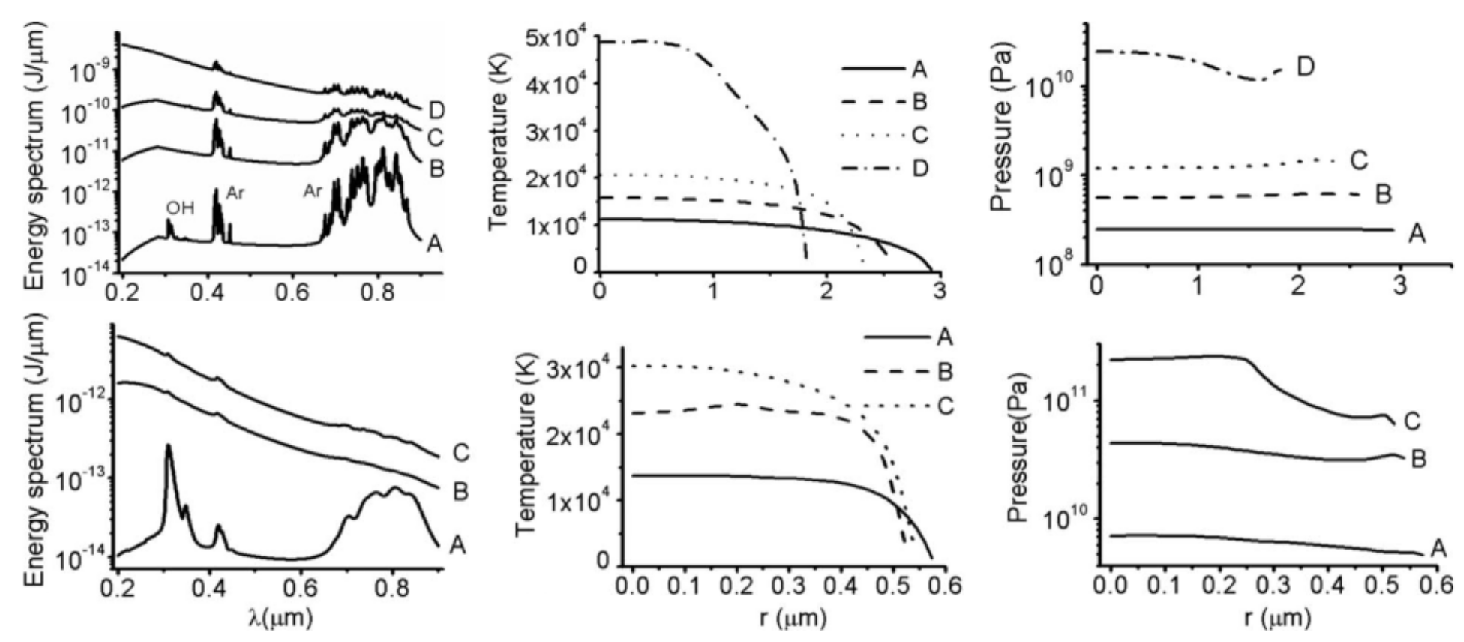
\includegraphics[width=0.9\linewidth]{figs/light.pdf}
    \caption{Simulations of an Ar bubble in 85\% aqueous H$_2$SO$_4$ (top-row) and in water (bottom-row). The gas Navier-Stokes equations were solved directly. The $1^{st}$ column shows the emitted spectrum as a function of wave-length, $\lambda$. The $2^{nd}$ and $3^{rd}$ columns shows the temperature and pressure as a function of position inside the bubble at the time the bubble is compressed to its minimum size. In the top row, the temperature was 20 $^o$C and the bubble was driven at $P_0$=1.5, 1.7, 2.0, and 4.0 atm for curves A, B, C, and D respectively. In the bottom row, A and B are driven at $P_0=$1.22 and 1.32 atm, respectively, at 20 $^o$C. Curve C is at $P_0$=1.32 atm and 0 $^0$C. All data are from ref. \cite{an2009diagnosing}.}
\label{fig:light}
\end{figure}

Let us first discuss SBSL of a \emph{pure} Ar bubble in water. Due to the absence of lines in SBSL spectra, early models only considered \emph{continuous} emission processes \cite{hilgenfeldt1999simple,hilgenfeldt1999sonoluminescence}. The derivations of the formulae for absorption coefficients are too long to fit in this paper, so we will simply highlight what is important; we include one of them as an example. At the very high temperatures that occur in the bubble ($\sim10,000-30,000$ K, see Fig. \ref{fig:light}), it is possible for electrons to become ionized from their atoms \cite{zel2002physics}. When a free electron passes near an ion, it is deflected by the Coulomb force. The electron is accelerated, changing its kinetic energy. Since the electron is charged, it emits radiation through bremsstrahlung \cite{jackson1999classical,griffiths2005introduction,zel2002physics}. A \emph{classical} expression for absorption due to electron-ion bremsstrahlung is derived in ref. \cite{zel2002physics} and is frequently used in the context of SBSL \cite{hilgenfeldt1999simple,hilgenfeldt1999sonoluminescence,an2006mechanism,an2008spectral,an2009diagnosing}:
\begin{equation}
    \kappa(\lambda,T(t)) = \frac{4}{3} \left( \frac{2\pi}{3 m_e k_B T(t)} \right)^{1/2} \frac{Z^2 e^6 \lambda^3}{ (4 \pi \epsilon_0)^3 h c^4 m_e } N_+ N_e .
    \label{eq:absorption_coeff}
\end{equation}
In eq. \ref{eq:absorption_coeff}, $m_e$ is the electron rest mass, $e$ is the elementary charge, $Z$ is the ``effective" charge of the ion (usually taken to be $Z=1$), $\epsilon_0$ is the vacuum permittivity, and $N_+$ and $N_e$ are, respectively, the number density of ions and electrons. Usually $N_+=N_e$ and $N_+N_e=N_e^2$. The fact that $\kappa \propto N_e N_+$ is intuitive: the amount of energy emitted/absorbed by electrons scattering off ions ought to be proportional to the number of electron and ions present. $N_e$ is easily calculated from the ``Saha equation" of astrophysics \cite{hilgenfeldt1999simple,an2006mechanism,zel2002physics}. Quantum mechanical calculations of $\kappa$ for electron-ion bremsstrahlung have also been done (see ref. for a review \cite{eckert2015aether}), but the formulae are considerably more complicated and are seldom used in the context of SBSL. If the electron becomes bound instead of being deflected, a different expression for the absorption has to be used \cite{zel2002physics}. The coefficient depends on which Ar atomic level the electron is in, but the free electron energy is continuous and electron-ion \emph{recombination} radiation is continuous, consistent with the continuous spectrum measured in water \cite{hilgenfeldt1999simple,hilgenfeldt1999sonoluminescence}. 

We're not done. It turns out that at the temperatures relevant to SBSL ($\sim 10^4$ K), the fraction of atoms that are ionized is only about $1\%$. The pressures that occur in SBSL ($\sim10^{12}$, see Fig. \ref{fig:light}) are so large that collisions between electrons and neutral atoms (which are otherwise rare) are frequent enough to be as important as electron-ion collisions \cite{zel2002physics,hilgenfeldt1999simple,frommhold1998electron}. A classical formula for the absorption coefficient for electron-atom bremsstrahlung is also available in ref. \cite{zel2002physics}, though more recent works \cite{an2006mechanism,an2008spectral,an2009diagnosing} use numerical results from quantum mechanical pseudopotential calculations \cite{geltman1973free}. 

Eq. \ref{eq:absorption_coeff}, combined with analogous formulae for electron-atom bremsstrahlung \cite{geltman1973free} and electron-ion recombination \cite{zel2002physics} were used to accurately calculate the spectrum of SBSL from Ar in water \cite{hilgenfeldt1999simple,hilgenfeldt1999sonoluminescence,hammer2002light,yasui2001effect,yasui1999mechanism}. The only remaining error was small disagreement in the number of photons emitted \cite{an2006mechanism}, which was later accounted for after SBSL was discovered in aqueous H$_2$SO$_4$ \cite{flannigan2005plasma,flannigan2005plasma1,flannigan2006measurement,suslick2008inside}. This later work discovered that emission \emph{lines} for Ar and Ar$^+$ excited state transitions [$\sim 400$ nm and $\sim 800$ nm, respectively, in Fig. \ref{fig:light} (left)] and continuous emission from electron-OH$^{+}$ recombination are present. However, at the conditions encountered in SBSL in water [Fig. \ref{fig:exp} (right)], the emission lines are concealed by the dominant continuum emission processes at high temperature while the electron-OH$^{+}$ recombination contribution diminishes as the remaining vapor content is driven out of the bubble at high pressure \cite{suslick2008inside,flannigan2005plasma,flannigan2005plasma1,flannigan2006measurement}. More recent calculations of SBSL in both water and aqueous H$_2$SO$_4$ that include all of these mechanisms are in excellent agreement with experiment, as can be seen by comparing Fig. \ref{fig:exp} and Fig. \ref{fig:light}. 

\section{Summary and Outlook}
We now have everything we need to describe SBSL will-nilly! We can use the RP equation, eq. \ref{eq:RP_2}, or one of it's variants to calculate the radius time curve, $R(t)$, of a bubble in SBSL. With a suitable model for the gas dynamics in the bubble (e.g. eq. \ref{eq:p_g}) the coupled RP and gas equations are solved numerically and fit to measured $R(t)$. This procedure allows us to ``measure" the temperature in the bubble. With $T(t)$, and knowing the correct mechanisms for emission/absorption in the bubble (which are electron-ion bremsstrahlung, electron-atom bremsstrahlung, and electron-ion recombination), we can calculate the radiated intensity as a function of time. The results of this procedure are the wave-length dependence of the emitted radiation, the pulse width (by solving as a function of time), and the number of photons (by integrating over the bubble and over time). The fact that all of these quantities are in excellent agreement with experiments has led to the popular opinion that SBSL is a ``solved" problem \cite{yasui2018acoustic,lohse2018bubble}.

It is interesting to note other distinct models for SBSL. A class of ``fractoluminescence" models have persisted in spite of the success of the work presented in this paper. These are based on the hypothesis that shape instabilities cause the bubble to violently disintegrate, resulting in velocities faster than the fluid can flow \cite{prosperetti1997new}. The fluid ``fractures" and plasma forms during dielectric breakdown across the fracture, emitting light \cite{borisenok2020mechanisms,borissenok2008sonoluminescence}. These models haven't gained much traction, however, since the requirement that the bubble disintegrates contradicts the fact that they don't...

An even more exotic theory supposes SBSL is from ``quantum vacuum radiation" \cite{schwinger1992casimir1,schwinger1992casimir2,schwinger1993casimir1,schwinger1993casimir2,schwinger1993casimir3,schwinger1993casimir4,schwinger1994casimir}. Schwinger proposed that shrinking a cavity would change the number of electromagnetic modes confined in it, changing the energy expectation value; the lost energy would be carried away by photons. Direct calculation of the number of photons was carried out by others \cite{eberlein1996sonoluminescence}. It was found that the number of emitted photons would be $10^{-10}$ times too small \cite{unnikrishnan1996comment,lambrecht1997comment,garcia1997comment,milton1996comment,liberati2000sonoluminescence}. The quantum vacuum radiation theory has been abandoned.

The theory discussed in this paper most likely explains \emph{shrimpoluminescence}, though some discrepancies should be addressed. The foremost being that shrimpoluminescence is too dim to be seen by the naked eye \cite{lohse2001snapping},  while SBSL in the lab is not. Recall that shrimpoluminescence is transient, while the theory developed in this paper is for stable bubbles. For a transient bubble, it is not possible for air molecules or water vapor to be ejected from the bubble, a process which occurs over $\sim10^3$ cycles. These extra degrees of freedom prevent the temperature from becoming as large as in \emph{stable} SBSL and the amount of emitted light is suppressed.
Another issue is that the bubble produced by a snapping shrimp is not stationary \cite{lohse1997sonoluminescing,versluis2000snapping}. Translating bubbles are not quite spherical \cite{brenner2002single}, and small shape distortions could decrease the peak pressure and temperature in the bubble, suppressing the amount of light produced \cite{matula2000single}. Still, the essential physics we have learned from SBSL in this paper at least gives us the tools we need to \emph{shine light} on shrimpoluminescence. 



%\raggedbottom

\bibliography{ref}

\end{document}
